\newpage
\section{Besoins fonctionnels}

$ \ast $ \textit{La section suivante pourra être négociée de manière à ce que toutes les parties prenantes soient en accord avec le contenu.} \\

La bête à corne ci-dessous permet de mieux comprendre les fonctions principales du projet, parties prenantes et objectifs du projet. \\
\label{ann:BeteCor}
\begin{figure}[h]
   \centering
   {
      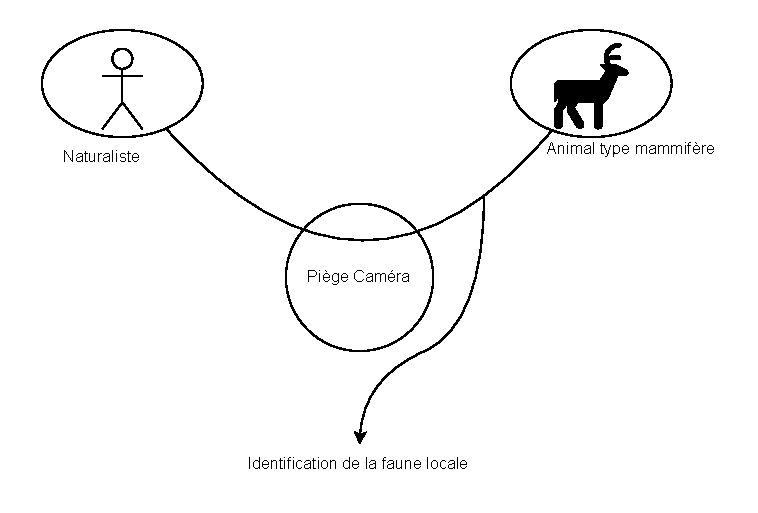
\includegraphics[width=0.7\textwidth]{images/bete_a_corne.pdf}
   }
   \caption{Bête à corne}
   \label{fig:BeteCor}
\end{figure}
\vspace{1.5em}

Au regard des besoins exprimés par le client, le projet s’inscrit dans une démarche de preuve de concept. L’objectif est de démontrer la faisabilité technique et opérationnelle d’un dispositif simplifié dans des conditions réelles, tout en maîtrisant les coûts et la complexité. Ce choix permet de concentrer les efforts sur un système fonctionnel, d’en valider les principes clés et de poser les bases pour d’éventuelles évolutions futures
\newline

Pour garantir la simplicité et la fiabilité du dispositif, nous proposons de déployer un unique piège caméra, dont la collecte initiale se limitera à la prise de photos, à l’horodatage et à la localisation GPS. Cette approche vise à optimiser la gestion énergétique et à réduire la complexité fonctionnelle.
\newline

L’architecture du système sera conçue de manière modulaire afin de permettre l’intégration ultérieure d’autres types de données, sans remettre en cause l’ensemble de l’infrastructure.
\newline

Les données seront transmises vers un stockage distant dès leur acquisition, sans traitement préalable dans le piège caméra. Cette méthode permet d’éviter les contraintes liées à la gestion d’un stockage local volumineux et à la récupération fréquente des cartes SD, tout en facilitant la logistique et en assurant un accès centralisé aux données.
\newline

Enfin, les données seront structurées sous forme tabulaire, afin de faciliter leur exploitation pour l’identification des espèces, conformément aux objectifs du projet.
\newline


Le système d’observation de la faune devra répondre à plusieurs besoins essentiels liés à sa mission principale : la collecte, la transmission et la mise à disposition des données sur les mammifères terrestres locales.


\small
\subsection{Fonctionnalités principales}
\begin{itemize}
   \item \textbf{Détection de mouvement animalier} : le dispositif doit détecter automatiquement la présence d’un animal dans son champ de vision.
   \item \textbf{Prise de vue automatique} : une photo doit être prise dès qu’un mouvement est détecté.
   \item \textbf{Enregistrement des images} : les clichés capturés sont enregistrés dans une mémoire locale avec leurs métadonnées (date, heure, température, position GPS).
   \item \textbf{Transmission des données} : les données collectées doivent être envoyées vers un stockage distant.
   \item \textbf{Autonomie énergétique} : le système, basé sur une batterie, doit être capable de fonctionner de manière autonome grâce à une gestion optimisée de la consommation d’énergie. Il devra également intégrer un mécanisme de surveillance permettant de suivre en temps réel la capacité énergétique restante, afin d’anticiper les besoins de recharge ou de maintenance.
\end{itemize}


\begin{center}
   \begin{tabular}{ | c || c | c | }
      \hline
      \textbf{Fonctionnalité}          & \textbf{Donnée}         & \textbf{Valeur nominale} \\ \hline
      Détection de mouvement animalier & Distance de détection   & 5 m                      \\ \hline
      Champs de Détection animalier    & Champs de détection     & 20 °                     \\ \hline
      Enregistrement de l'image        & Qualité de l'image      & 480p                     \\ \hline
      Autonomie énergétique            & Durée de fonctionnement & 24 h                     \\ \hline
   \end{tabular}
\end{center}


\subsection{Fonctionnalités supplémentaires ou optionnelles}
\begin{itemize}
   \item \textbf{Interface utilisateur Web} : une interface simple et ergonomique doit permettre la consultation des données (photos, localisation, informations environnementales, etc ...).
   \item \textbf{Traitement des images} : Un module de reconnaissance visuelle permettra d’identifier les espèces photographiées.
   \item \textbf{Visualisation et analyse des données} : la page Web pourra afficher des graphiques, cartes interactives et calendriers d’observation.
   \item \textbf{Acquisitions de données environnementales supplémentaires} : Ajouts d’autres mesures via divers moyen (pression atmosphérique, CO$_2$, qualité de l’air, humidité, son, etc.).
   \item \textbf{Gestion énergétique améliorée} : intégration d’un moyen de recharge afin de prolonger la durée d’utilisation du système et d’optimiser son indépendance énergétique sur le terrain.
\end{itemize}

